\documentclass[../main/main.tex]{subfiles}

\newdate{date}{23}{09}{2020}

% \begin{figure}[h!]
% \centering
% \includegraphics[page=6,width=0.8\textwidth]{../lessons/pdf_file/02_lecture.pdf}
% \end{figure}

%\displaydate{date}. Compiled:  \today. Alice.

\begin{document}

\pagestyle{plain}

\section{Lecture 2}


\subsubsection*{Slide 1}

\begin{minipage}[]{0.5\linewidth}
\centering
\includegraphics[page=1,width=1\textwidth]{../lessons/pdf_file/02_lecture.pdf}
\end{minipage}
\hspace{0.3cm}\vspace{0.3cm}
\begin{minipage}[c]{0.47\linewidth}
Now, we will talk about different kinds of polarization that we have. Let us start with the \textbf{linear polarization}: if the amplitude of the electric field is a real vector, we have a linear polarized wave, so the orientation of that vector represents the direction of polarization of your linearly polarized way. For instance, this is a snap of the electromagnetic way at time \( t=0 \). For the different positions, the electric field is still oriented along the \( x \) axis.
\end{minipage}

\subsubsection*{Slide 2}

\begin{minipage}[]{0.5\linewidth}
\centering
\includegraphics[page=2,width=1\textwidth]{../lessons/pdf_file/02_lecture.pdf}
\end{minipage}
\hspace{0.3cm}\vspace{0.3cm}
\begin{minipage}[c]{0.47\linewidth}
This is the same wave at position \( z=0 \) as a function of time. It is oscillating but mantains the oscillations along the \( x \) axis. Conventionally, when we talk about polarization we refer to the orientation of electric field.
\end{minipage}

\subsubsection*{Slide 3}

\begin{minipage}[]{0.5\linewidth}
\centering
\includegraphics[page=3,width=1\textwidth]{../lessons/pdf_file/02_lecture.pdf}
\end{minipage}
\hspace{0.3cm}\vspace{0.3cm}
\begin{minipage}[c]{0.47\linewidth}
For a linearly polarized way, the electric field always mantains the direction with respect of the axis. In this case, we have a linearly polarized wave forming an angle of 135° with respect to the \( x \) axis. The amplitude changes becuase it is still oscillating along this axis. To recap: if the vector that desribes the electric field amplitude \( \va{E_0} \) is a real one, we have a linearly polarized wave and the angles define the orientation of the polarization.
\end{minipage}

\newpage

\subsubsection*{Slide 4}

\begin{minipage}[]{0.5\linewidth}
\centering
\includegraphics[page=4,width=1\textwidth]{../lessons/pdf_file/02_lecture.pdf}
\end{minipage}
\hspace{0.3cm}\vspace{0.3cm}
\begin{minipage}[c]{0.47\linewidth}
Let us suppose that we overlap two linearly polarized way in orthogonal orientations. We are introducing a phase shift \( \delta  \) to the \( y \) component with respect to the \( x \) component. We obtain a \textbf{right-circularly polarized (R)} wave:
\begin{equation*}
  E_{0x} = E_{0y} \quad \delta = -\frac{\pi }{2}
\end{equation*}
The vector that describe the polarization, does not mantain the same orientation along the plane, but the tick of the arrow is rotating in the \textbf{clockwise} direction.
It is still again a convention-
\end{minipage}

\subsubsection*{Slide 5}

\begin{minipage}[]{0.5\linewidth}
\centering
\includegraphics[page=5,width=1\textwidth]{../lessons/pdf_file/02_lecture.pdf}
\end{minipage}
\hspace{0.3cm}\vspace{0.3cm}
\begin{minipage}[c]{0.47\linewidth}
If the phase shift is:
\begin{equation*}
  E_{0x} = E_{0y} \quad \delta = +\frac{\pi }{2}
\end{equation*}
we have a \textbf{counter-clockwise} rotation (looking from the receiver).
\end{minipage}

\subsubsection*{Slide 6}

\begin{minipage}[]{0.5\linewidth}
\centering
\includegraphics[page=6,width=1\textwidth]{../lessons/pdf_file/02_lecture.pdf}
\end{minipage}
\hspace{0.3cm}\vspace{0.3cm}
\begin{minipage}[c]{0.47\linewidth}
If we start with two linearly polarized waves but with different amplitudes and we have a given shift, we will end up with:
\begin{itemize}
    \item \textbf{right-elliptically} polarized wave (\textbf{(R)}):
    \begin{equation*}
      E_{0x} \neq E_{0y} \quad \delta = - \frac{\pi }{2}
    \end{equation*}

    \item \textbf{left-elliptically} polarized wave (\textbf{(L)}):
    \begin{equation*}
      E_{0x} \neq E_{0y} \quad \delta = + \frac{\pi }{2}
    \end{equation*}
\end{itemize}

\end{minipage}

\newpage

\subsubsection*{Slide 7}

\begin{minipage}[]{0.5\linewidth}
\centering
\includegraphics[page=7,width=1\textwidth]{../lessons/pdf_file/02_lecture.pdf}
\end{minipage}
\hspace{0.3cm}\vspace{0.3cm}
\begin{minipage}[c]{0.47\linewidth}
We can generalize this idea. In general, if we sum up two components, we can have different situations accordingly to the relative phase shift. If \( E_{0x} \neq E_{0y} \), you cannot get circular polarized waves.
\end{minipage}

\subsubsection*{Slide 8}

\begin{minipage}[]{0.5\linewidth}
\centering
\includegraphics[page=8,width=1\textwidth]{../lessons/pdf_file/02_lecture.pdf}
\end{minipage}
\hspace{0.3cm}\vspace{0.3cm}
\begin{minipage}[c]{0.47\linewidth}
How is it physically possible to obtain a linear polarized wave? Let us consider the sun's light (which we consider \emph{unpolarized} and that is represented by a convolution of arrows along all directions).
A \textbf{Linear polarizer} gives you a linearly polarized wave along the \textbf{trasmission axis} (it blocks completely all the waves that are linearly polarized along the orthogonal direction of the trasmission axis).

In reality, the most cheap object is the \textbf{polaroid film}, which contains molecules which have an absorbtion which select highly to the orientation. They work perfectly as a linear polarizer. Sunglasses are made with polaroid films.
\end{minipage}

\subsubsection*{Slide 9}

\begin{minipage}[]{0.5\linewidth}
\centering
\includegraphics[page=9,width=1\textwidth]{../lessons/pdf_file/02_lecture.pdf}
\end{minipage}
\hspace{0.3cm}\vspace{0.3cm}
\begin{minipage}[c]{0.47\linewidth}
Let us suppose to have non polarized ligth, a polarizer and then we use the second polarizer as an analyzer (we rotate it with respect to the trasmission axis of the first polarizer). We are just making the projection of the beam along the polarizer. The component we obtain is \( E_0 \cos(\theta )  \) (where \( \theta  \) is the relative angle between the two trasmission axis).
The \textbf{Malus law} (1809) is:
\begin{equation*}
  I(\theta ) = I_0 \cos^2(\theta )
\end{equation*}
which is the intensity coming from an analyzer. If we use just one polarizer, (\textbf{unpolarized beam}) we can describe this still using Malus law: in this case we are taking an average over all the possible orientations:
\begin{equation*}
  I = \frac{1}{2} I_0 \rightarrow T = \frac{1}{2}
\end{equation*}

\end{minipage}

\subsubsection*{Slide 10}

\begin{minipage}[]{0.5\linewidth}
\centering
\includegraphics[page=10,width=1\textwidth]{../lessons/pdf_file/02_lecture.pdf}
\end{minipage}
\hspace{0.3cm}\vspace{0.3cm}
\begin{minipage}[c]{0.47\linewidth}
We can consider also the situation in we have a partial degree of linear polarization and we can quantify the \textbf{degree of polarization}, by using a polarizer. If you want to determine \( G \) experimentally, you have the analyzer rotating in from fo your beam and you measure the maximum and the minimum.
\end{minipage}

\subsubsection*{Slide 11}

\begin{minipage}[]{0.5\linewidth}
\centering
\includegraphics[page=11,width=1\textwidth]{../lessons/pdf_file/02_lecture.pdf}
\end{minipage}
\hspace{0.3cm}\vspace{0.3cm}
\begin{minipage}[c]{0.47\linewidth}
Let us try to make an example using the linearly polarized beam.
\end{minipage}

\subsubsection*{Slide 12}

\begin{minipage}[]{0.5\linewidth}
\centering
\includegraphics[page=12,width=1\textwidth]{../lessons/pdf_file/02_lecture.pdf}
\end{minipage}
\hspace{0.3cm}\vspace{0.3cm}
\begin{minipage}[c]{0.47\linewidth}
Let us do a different exercise.
\end{minipage}

\subsubsection*{Slide 13}

\begin{minipage}[]{0.5\linewidth}
\centering
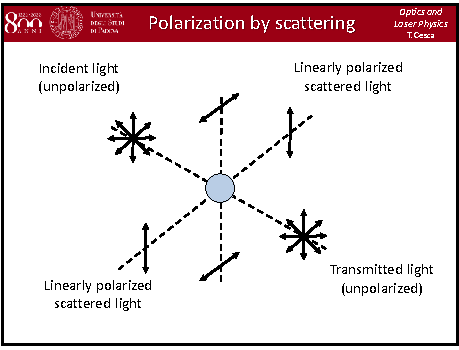
\includegraphics[width=1\textwidth]{../lessons/pdf_file/02/02_S13.pdf}
\end{minipage}
\hspace{0.3cm}\vspace{0.3cm}
\begin{minipage}[c]{0.47\linewidth}
In reality, when is it possible to get a polarized beam? The simplest situation is light scattered from the atmosphere (so ligth coming from the sun is not completely unpolarized, it has a degree of polarization by scaterring with molecules of the atmosphere). With a very simple description we consider molecules of the atmosphere as electric dipoles. Like for electric dipoles, the degree of polarization will be maximum along the direction perpendicular to the direction of ligth. We start from unpolarized incident light, the trasmitted light along the same direction is still unpolarized. But in the orthogonal direction, you will get the maximum degree of polarization.
\end{minipage}

\subsubsection*{Slide 14}

\begin{minipage}[]{0.5\linewidth}
\centering
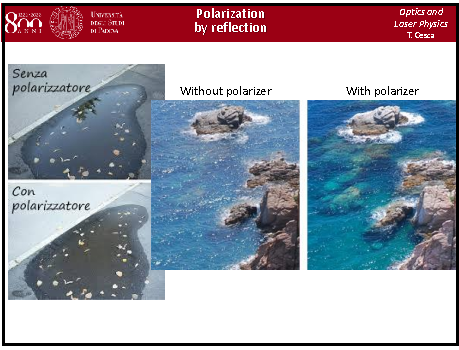
\includegraphics[width=1\textwidth]{../lessons/pdf_file/02/02_S14.pdf}
\end{minipage}
\hspace{0.3cm}\vspace{0.3cm}
\begin{minipage}[c]{0.47\linewidth}
Sunglasses are polarized because you can reduce a lot the reflection components (the reflected beam is typically partially polarized).
\end{minipage}

\subsubsection*{Slide 15}

\begin{minipage}[]{0.5\linewidth}
\centering
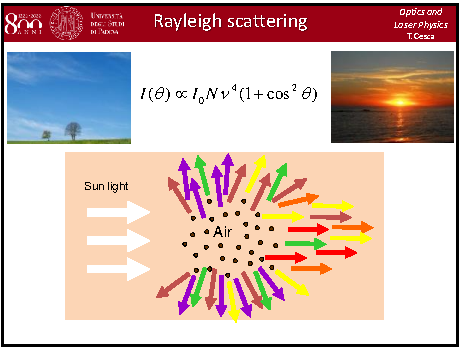
\includegraphics[width=1\textwidth]{../lessons/pdf_file/02/02_S15.pdf}
\end{minipage}
\hspace{0.3cm}\vspace{0.3cm}
\begin{minipage}[c]{0.47\linewidth}
Let us consider particles that compose atmosphere. Why is the sky blue? The reason is related to scattering. The intensity scattered by molecus on the atmosphere has this dependence (see equation) from the angle (of the ligth) and the frequency. Light is scattered from atmosphere from all the possible orientation: the intensity is strongly dependent on \( \nu ^4 \). The highest intensity is for the component with the highest frequency (blue region). That is why when we are averaging over all the possible orientation, the components which we recevie most are the component on the blue region.

The situation is completely different if we look at the sky during sunset (sun is close to horizon): the light is moving parallel to the surface. Actually, light which reach our eyes is on the component which is not scattered in different directions, i.e. yellow.

\end{minipage}

Hence, the intensity of the component that are scattered in different direction are much higher for blue components than for the red component.



\end{document}
